\documentclass{standalone}
\usepackage{tikz}
\usepackage{ctex,siunitx}
\setCJKmainfont{Noto Serif CJK SC}
\usepackage{tkz-euclide}
\usepackage{amsmath}
\usetikzlibrary{patterns, calc}
\usetikzlibrary {decorations.pathmorphing, decorations.pathreplacing, decorations.shapes,}

\begin{document}
\small
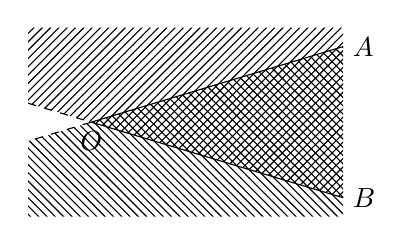
\begin{tikzpicture}[>=stealth,scale=0.8]
  \tkzSetUpPoint[fill=black]
  % \useasboundingbox(-1,-0.75)rectangle(3.7,1.4);
  \draw[dashed](-1,.3)--(0,0)--(-1,-.3);
  \draw(4,-1.2)node[right]{$B$}--(0,0)node[below]{$O$}--(4,1.2)node[right]{$A$};
  \fill[pattern=north east lines](-1,.3)--(-1,1.5)--(4,1.5)--(4,-1.2)--(-1,.3);
  \fill[pattern=north west lines](-1,-.3)--(-1,-1.5)--(4,-1.5)--(4,1.2)--(-1,-.3);
\end{tikzpicture}
\end{document}